\documentclass[conference]{IEEEtran}
\usepackage{amsmath, amsthm, amssymb, fancyhdr, enumerate}
\usepackage[tight,footnotesize]{subfigure}
\ifCLASSINFOpdf
\usepackage[pdftex]{graphicx}
\graphicspath{{../poster/images/}}
\else
\usepackage[dvips]{graphicx}
\graphicspath{{../poster/images/}}
\fi


\hyphenation{op-tical net-works semi-conduc-tor}

\begin{document}

\title{Unsupervised Spike Sorting}

\author{
\IEEEauthorblockN{David Brody}
\IEEEauthorblockA{Department Of Computer Science \\
Stanford University\\
Stanford, California 94305}
\and
\IEEEauthorblockN{Daniel Sommerman}
\IEEEauthorblockA{Department Of Computer Science \\
Stanford University\\
Stanford, California 94305}
\and
\IEEEauthorblockN{Michael Gummelt}
\IEEEauthorblockA{Department Of Computer Science \\
Stanford University\\
Stanford, California 94305}
}


\maketitle
\begin{abstract}
In this paper, we outline our approach to automatic spike sorting in the
context of electrical response from neurons. Using compression techniques
such as PCA and polynomial approximations, we were able to find a
tractable subspace in which to analyze our features. On our reduced
dimension samples, we then applied two algorithms wrapping k-means which
help find k: g-means clustering and using the Davies-Bouldin index. We
were able to get some 
very good clusters while other clusters were not as well separated,
indicating that there was a combination of a large degree of noise in our
features and high variability in terms of the response of each sensor when
a single cell spikes.
\end{abstract}

\IEEEpeerreviewmaketitle


\section{Introduction}

Lab equipment gathers extracellular neurophysicological voltage samples at
a rate of 10 kHz. These readings are a mixture of the responses from the
many surrounding cells. The responses are then clustered into
similar shaped groups which represent different cells. Our
project aims to take this analysis step which is usually done
manually and automate it using machine learning. The data is 100
seconds of recorded retinal ganglion cell responses. The data is
extracellular recordings from 60 different channels. Each channel 
represents a data stream of voltage potentials at a specific
microelectrode.
\vskip1em
\begin{center}
\centering
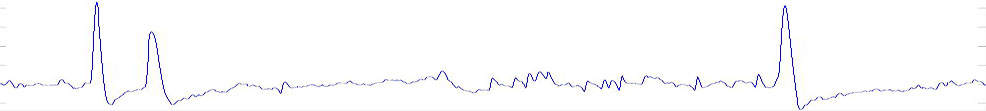
\includegraphics[width=0.6\linewidth]{voltagetrace_2_small.jpg}\\
\small{Example microelectrode recording.}
\label{fig_sim}
\end{center}

The aim of the project is to cluster each spike into clusters
which each share a similar shape. 

\begin{center}
  \begin{tabular}{c c c}
    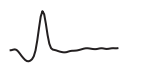
\includegraphics[width=0.17\linewidth]{WaveShape1.png} &
    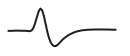
\includegraphics[width=0.17\linewidth]{WaveShape2.png} &
    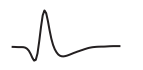
\includegraphics[width=0.17\linewidth]{WaveShape3.png}
  \end{tabular}
  \\
  \small{Example single channel cluster center shapes}
\end{center}

\section{Algorithmic Exploration}
\subsection{Model}
\noindent{\textbf{Model Parameters}}

N = \# of datapoints per channel

CH = \# of channels

S = \# of points to smooth raw data over

T = Threshold for spikes

L = \# points to take from left of spike location

R = \# points to take from right of spike location

\noindent{\textbf{Definitions}}
We begin with the raw waveform:
$$R = \{ {R \in \mathbb{R}^{N \times CH}; i = 1,...,CH} \}$$
Smoothing over S points we define a new waveform where $R^i_j$
is the jth datapoint in the ith channel: 
$$W^i_j = \frac{1}{s}\sum_{s=-S/2}^{S/2}R^{(i)}_{j+s}$$
We then define $W'$ as the zero mean normalized to the standard
deviation on each channel of $W$. The next step is to
separate out the possible spikes to cluster. We define the
spike locations of interest as:
$$P = \{ i; \frac{\partial}{\partial W} = 0 \cap 
  (W_1'(P_i) > T \cup ... \cup W_{CH}'(P_i) > T) \cap i \in
  1,...,N \} $$
This represents any point that is a local maximum and is above the
threshold $T$ on any channel. Peaks are then cut to ensure that they are a minimum of
$\alpha = 15$ from each other. To form a single feature vector $X^{(i)}$ we take the
 surrounding points on each channel and concatentate them.
 $$X^{(i)}_j = W'^{floor(i/(L+R+1))+1}_{mod(j, L+R+1) + P(i)}
  ; i = 1,...,|P|, j = 1,...,(L+R+1)*CH$$
  $$X^{(i)} \in \mathbb{R}^{CH(L+R+1)}$$
$X$ is the feature vector we use to then cluster on.

\subsection{Process Overview}

For reference, the high level overview of our process pipeline is shown
below: 
\begin{center}
  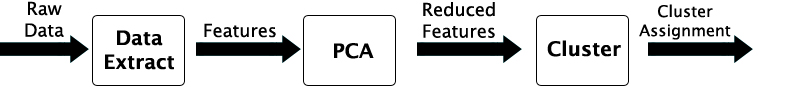
\includegraphics[width=0.8\linewidth]{../poster/images/pipeline.jpg}
\end{center}

We paramaterize our feature vectors from the raw data with the following representations:
$$X = M(R; S,T,L,R)$$
We then use different methods to reduce the dimensionality of
the feature vectors to improve performance and to emphasize
more discrimanent features.

$$Red(X, N, M; X^{(i)} \in \mathbb{R}^N) = Y; Y^{(i)} \in \mathbb{R}^M$$

Clustering then takes the dimension reduced feature vectors
and assigns them to clusters which represent possible cells.

 $$Clus(X; X^{(i)} \in \mathbb{R}^M) = (Y^{(i)} \in
  \mathbb{R}^M,I^{(i)} \in \mathbb{R})$$

\subsection{Dimensionality reduction and compression}
\subsubsection{PCA}
At this point, we have our features and are ready to run unsupervised
learning algorithms on the data set. However, as we began experimenting
with our data set, we realized that the time needed to learn on our data
set was simply too great. We needed a way to reduce the dimensionality of
our features. Since a feature vector consists of 30 measurements for 60
channels each, we have features in $\mathbb{R}^{1800}$.

The first approach we took was to apply PCA. Figure 2 shows the error
versus target dimensions reduced to. Factoring in compression and
percentage of error, 300 principal components optimizes both.
We then take the components and project our features into that space, $\mathbb{R}^{300}$.

Performing this optimization allowed us to run k-means clustering in 13\%
of the time without compression. This significantly reduces the time
needed without sacrificing too much in terms of underfitting. Figure 1
shows the relationship between the dimensionality of our
featuer vectors and the time it takes to run our clustering code. As we
iterated on our project, reducing the running time of our algorithm was
critical to being able to try many different ideas quickly.

\begin{figure}
\centering
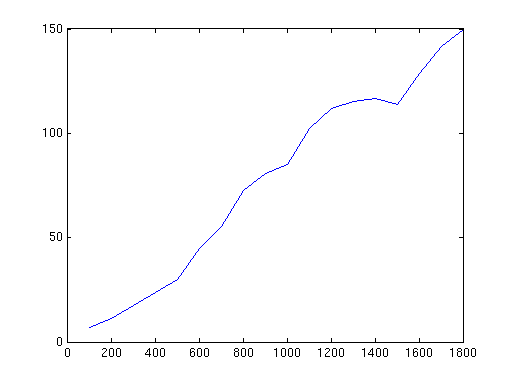
\includegraphics[width=3in,height=2in]{../poster/images/dim_vs_runningtime.png} 
\caption{This plot of the time clustering took (using g-means) vs the
  dimension we reduced to using PCA shows the roughly linear relationship 
between dimensionality of our feature vector and running
time.}
\end{figure}

\subsubsection{Fitting Polynomials}

Another approach to reducing the dimensionality was to take
into account the dependencies of the features within each
channel. Since these values are continuous we can fit a
polynomial model to them with fewer parameters. Here we let $n$
be the number of coefficients we want to fit per channel. Since
we have 60 channels the end result is $\mathbb{R}^{60(n+1)}$
since the intercept parameter must be included per channel as well.

Our results with polynomial fitting were not as strong as
PCA. While they do a good job of making sure each channel is
fit well, the condensed features must encode all the
information unlike PCA where the principle components hold the
information. As a result, it takes many more features to get
the same amount of information back.

\begin{figure}
\centering
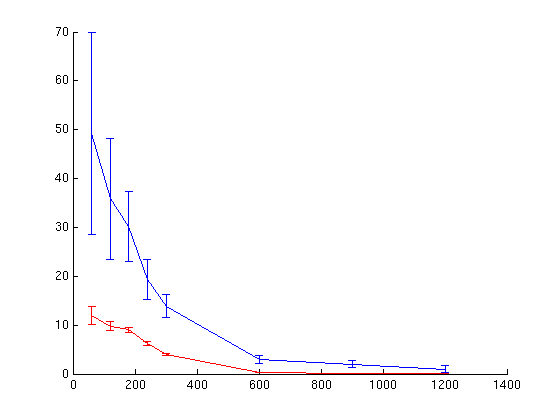
\includegraphics[width=3in,height=2in]{../poster/images/error_poly_pca.png}
\caption{This plot compares the error of the compression techniques we
  used. In blue is polynomial fitting and in red is PCA. The plot is of
  the percentage error vs dimension we reduce to.}
\end{figure}

While polynomial fitting does take temporal information into
account per channel in the condensation, it fails to encode the
meaningful information as well.

\subsection{Clustering Algorithms}
As the engine for both of the clustering algorithms, we used kmeans
clustering. However, the real work at this stage is to determine which k
should be used in kmeans. We tried two approaches to solving this
problem. 

\subsubsection{G-Means algorithm}
One way to choose k in the k-means algorithm is to use an algorithm
developed in 2003 by Greg Hamerly and Charles Elka, presented in the NIPS
2003 conference \cite{gmeans}. In this method, a small value for k is
chosen and kmeans is run. Then, for each cluster produced, we use a
heuristic function to decide whether to split that cluster. The heuristic
used is the Anderson-Darling statistic. If that statistic is greater than
some threshold critical value, then we decide that the cluster should be
split. The Anderson-Darling statistic is computed as follows:
$$
A^2(Z) = -n - \frac{1}{n}\sum_{i=1}^n (2i -
1)[\log(z_i)+\log(1-z_{n+1-i})]
$$$$
A^2_*(Z) = A^2(Z)(1 + 4/n - 25/n^2)
$$
If the $A^2_*(Z)$ is greater than the threshold, we split. For this
project we experimented with many thresholds and found that with $t=12$ we
got good separation between clusters.

\begin{figure}
\centering
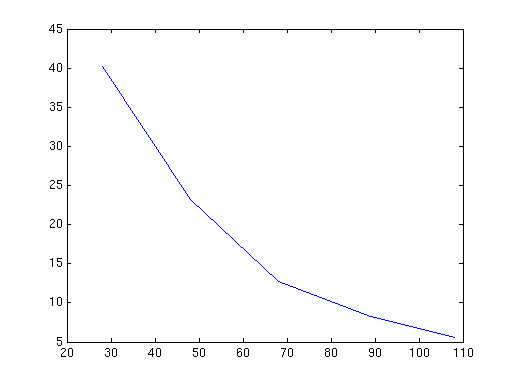
\includegraphics[width=1.3in,height=1in]{../poster/images/gmeans_k_vs_metric.png} 
\caption{The Anderson-Darling statistic is computed per cluster, so to
  show how it improves, we take the average value across all clusters and
  for each $k$ plot the mean here.}
\end{figure}


\subsubsection{Davies-Bouldin Index}
The DB Index is
another way to determine $k$ by favoring sets of clusters
with high intra-cluster similarity and low inter-cluster
similarity.  The formula is as follows:

$A^j$ = Center of cluster j

$T^j = \{ {X^{(i)} ; X^{(i)} \text{is in cluster} j} \}$

$S^i$ = the intra cluster similarity of cluster $i$

$M^{ij}$ = inter cluster similarity of clusters $i$, $j$

$S^i = (\frac{1}{|T^i|} \sum\limits_{j=1}^{|T^i|} (T^i_j -A^i)^q)^{\frac{1}{q}}$

$M^{ij} = (\sum\limits_{k=1}^{N} |a^i_k - a^j_k|^p)^{\frac{1}{p}}$

$DB = \frac{1}{N} \sum\limits_{i=1}^N \max_{j:i \neq j} R_{ij}$

\begin{figure}
\centering
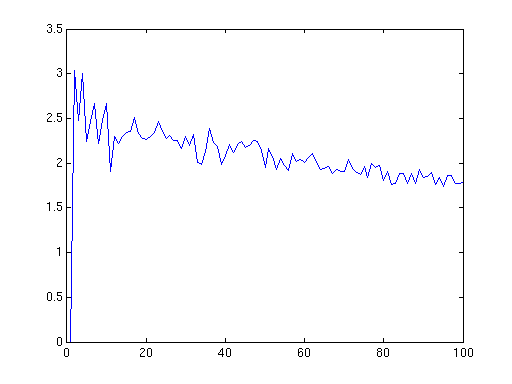
\includegraphics[width=1in,height=1in]{../poster/images/davies_k_vs_davies_index.png}
\caption{The graph above shows k vs the Davies-Bouldin Index}
\end{figure}

%\begin{figure*}
%\centering
%
\includegraphics[width=1in,height=1in]{sns.jpg}
%\caption{A sample black and white graphic (.eps format)
%that needs to span two columns of text.}
%\end{figure*}

\section{Results}

The results are clusters that each represent a unique
waveform shape. However, while these clusters are unique, there is no
guarantee if they are correct cells are not. Since this is
unsupervised learning further analysis with the stimulus would be
needed to see how clean these cells are.

Looking at how the clusters lay out we see that many clusters have few
points within them. These could be far away cells that can be
separated out but it is hard to tell over the noise of the system. We
compare the different methods of obtaining features and see that on
the mostpart they result in a similar distribution of cluster sizes(Fig. 5.).

\begin{figure}
\centering
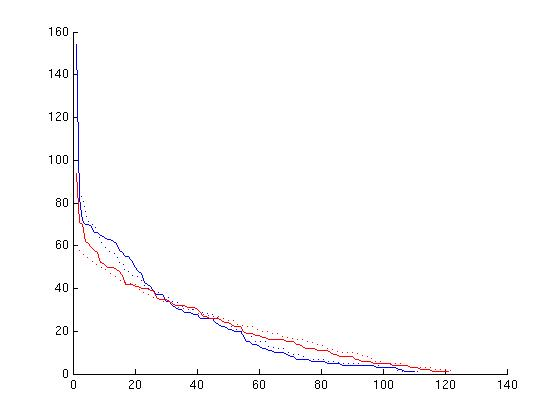
\includegraphics[width=0.9\linewidth]{traces/clusthistcount.jpg}
\caption{Shows the number of samples in each cluster sorter. Red is
  PCA and blue is polyfit. Dashed is L=8, R= 21; Solid is L = 21, R = 8.}
\end{figure}

Next we look at how the clusters compare with each other.  To view the
results, the top 3 clusters were chosen. Taking the top two
principle components of the combined data from the clusters and then
plot each $X^{(i)}$ within this space gives these plots. Each point is colored for its
cluster. First we compare how different parameters for forming the
features compare by adjusting R and L. We see that having features
more based on what is after the spike leads to more separable
datapoints (Fig. 7 and 9 versus Fig 6 and 8). We also see that PCA
does better than polyfit not only in that the clusters are more
separable but also PCA gets more
datapoints in the top clusters (Fig. 10 and 11). Furthermore, taking the top five
clusters within a three dimensional space using the top three
priciples componenets, we see they also mostly separate (Figure. 12).

\begin{figure}
\centering
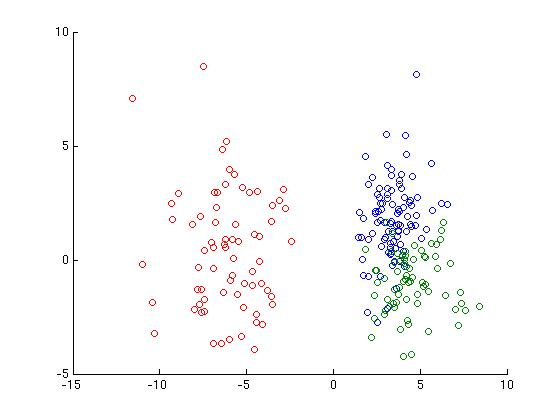
\includegraphics[width=0.7\linewidth]{plots/poly_L.jpg}
\caption{Top three clusters using polynomial features. L = 21, R = 8.}
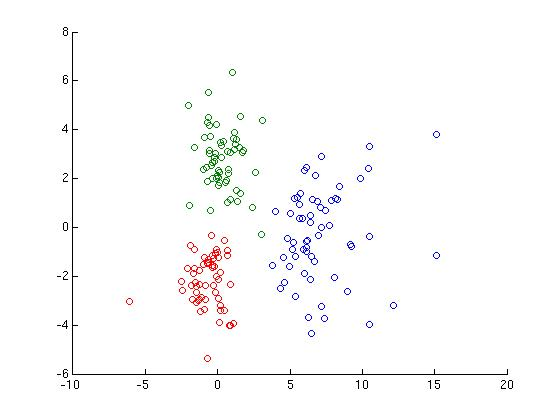
\includegraphics[width=0.7\linewidth]{plots/poly_R.jpg}
\caption{Top three clusters using polynomial features. L = 8, R = 21.}
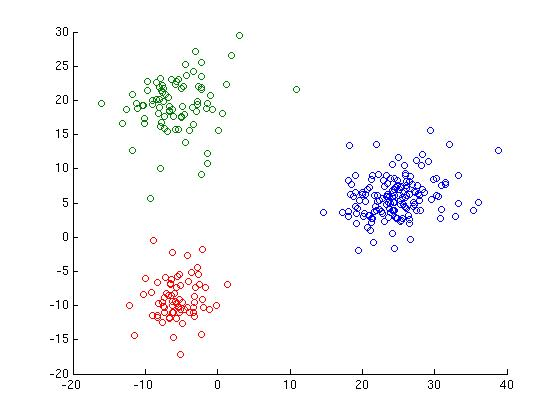
\includegraphics[width=0.7\linewidth]{plots/PCA_L.jpg}
\caption{Top three clusters using PCA features. L = 21, R = 8.}
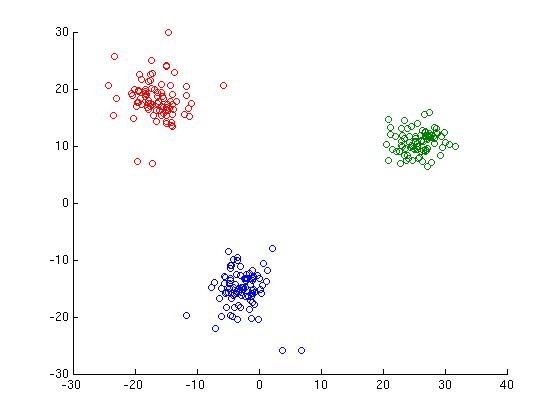
\includegraphics[width=0.7\linewidth]{plots/PCA_R.jpg}
\caption{Top three clusters using PCA features. L = 8, R = 21.}
\end{figure}

\begin{figure}
\centering
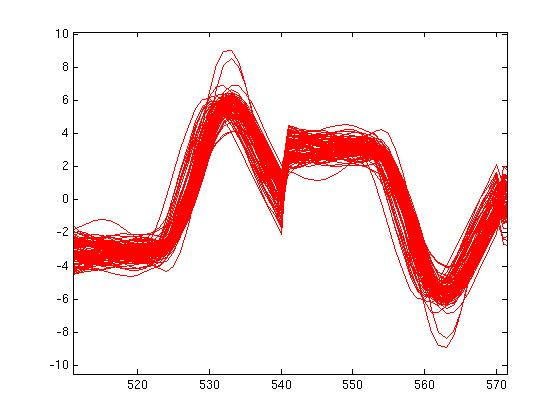
\includegraphics[width=0.7\linewidth]{traces/clustertrace_pca_front.jpg}
\caption{Traces of top cluster using PCA. Top two channels.}
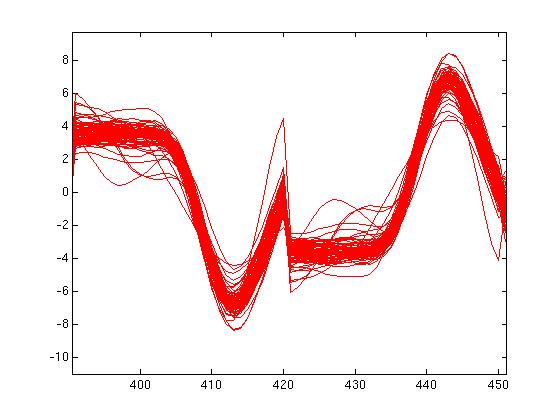
\includegraphics[width=0.7\linewidth]{traces/clustertrace_poly_front.jpg}
\caption{Traces of top cluster using Polynomial fitting. Top two
  channels.}
\end{figure}

\begin{figure}
\centering
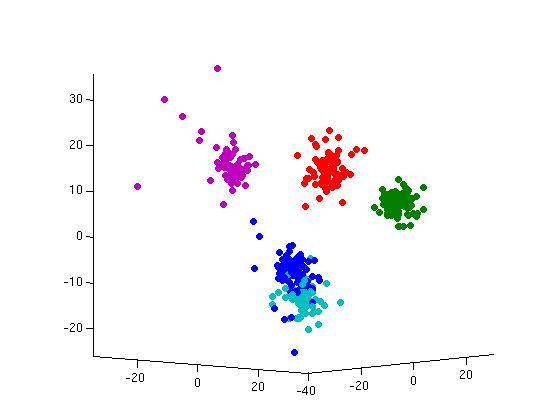
\includegraphics[width=0.7\linewidth]{traces/pca_top5_3d.jpg}
\caption{Top 5 clusters using PCA transformed into three dimensional
  space using top three principle components.}
\end{figure}




\section{Conclusions}
We found PCA to be very useful to compress the data so we could work
in a high dimension more efficiently. However, understanding the
meaning of the data and how to format it correctly is important when
forming features. We also found clustering to be challenging since the
number of clusters and the confidence of them is very dependent on the
heuristic used.  Lastly, this highlights the challenge in performing
unsupervised learning with real world data.

\subsection{Future Work}
Future work within this space could be to try using scale and
translation independent encoding of the waveforms. This could make the
algorithm less sensitive to variations.  We also believe there could
be better clustering algorithms to take specific physiological 
aspects into account.


\section*{Acknowledgment}
The authors would like to thank the Stephen Baccus Lab for providing
the data and the insight into how to approach this problem.


%\end{document}  % This is where a 'short' article might terminate
\begin{thebibliography}{1}


\bibitem{IEEEhowto:kopka}
UCSD, \emph{Spike Sorting},
http://physics.ucsd.edu/neurophysics/publications/obd\_ch3\_2.pdf

\bibitem{IEE}
M. Lewicki, \emph{A review of methods for spike sorting}
http://www.tsolab.org/jclub/20090429/lewicki.pdf

\bibitem{ee}
D. Davies, D. Bouldin, \emph{A cluster separation measure}
http://ieeexplore.ieee.org/xpls/abs\_all.jsp?arnumber\=4766909\&tag\=1


\end{thebibliography}

\end{document}
